\chapter{Implementation}

\section{Current Implementation of Dynamic Action Discovery in ASP.NET Core}

Web applications primarily respond to user requests, and while hardcoding each endpoint and its response would theoretically serve this purpose, it's not a practical solution when dealing with hundreds of endpoints. ASP.NET Core handles this challenge by using controllers—classes that group related actions and automate endpoint mapping through attributes. Figure \ref{fig:controller} illustrates an example of such a controller.

\begin{figure}[H]
\centering
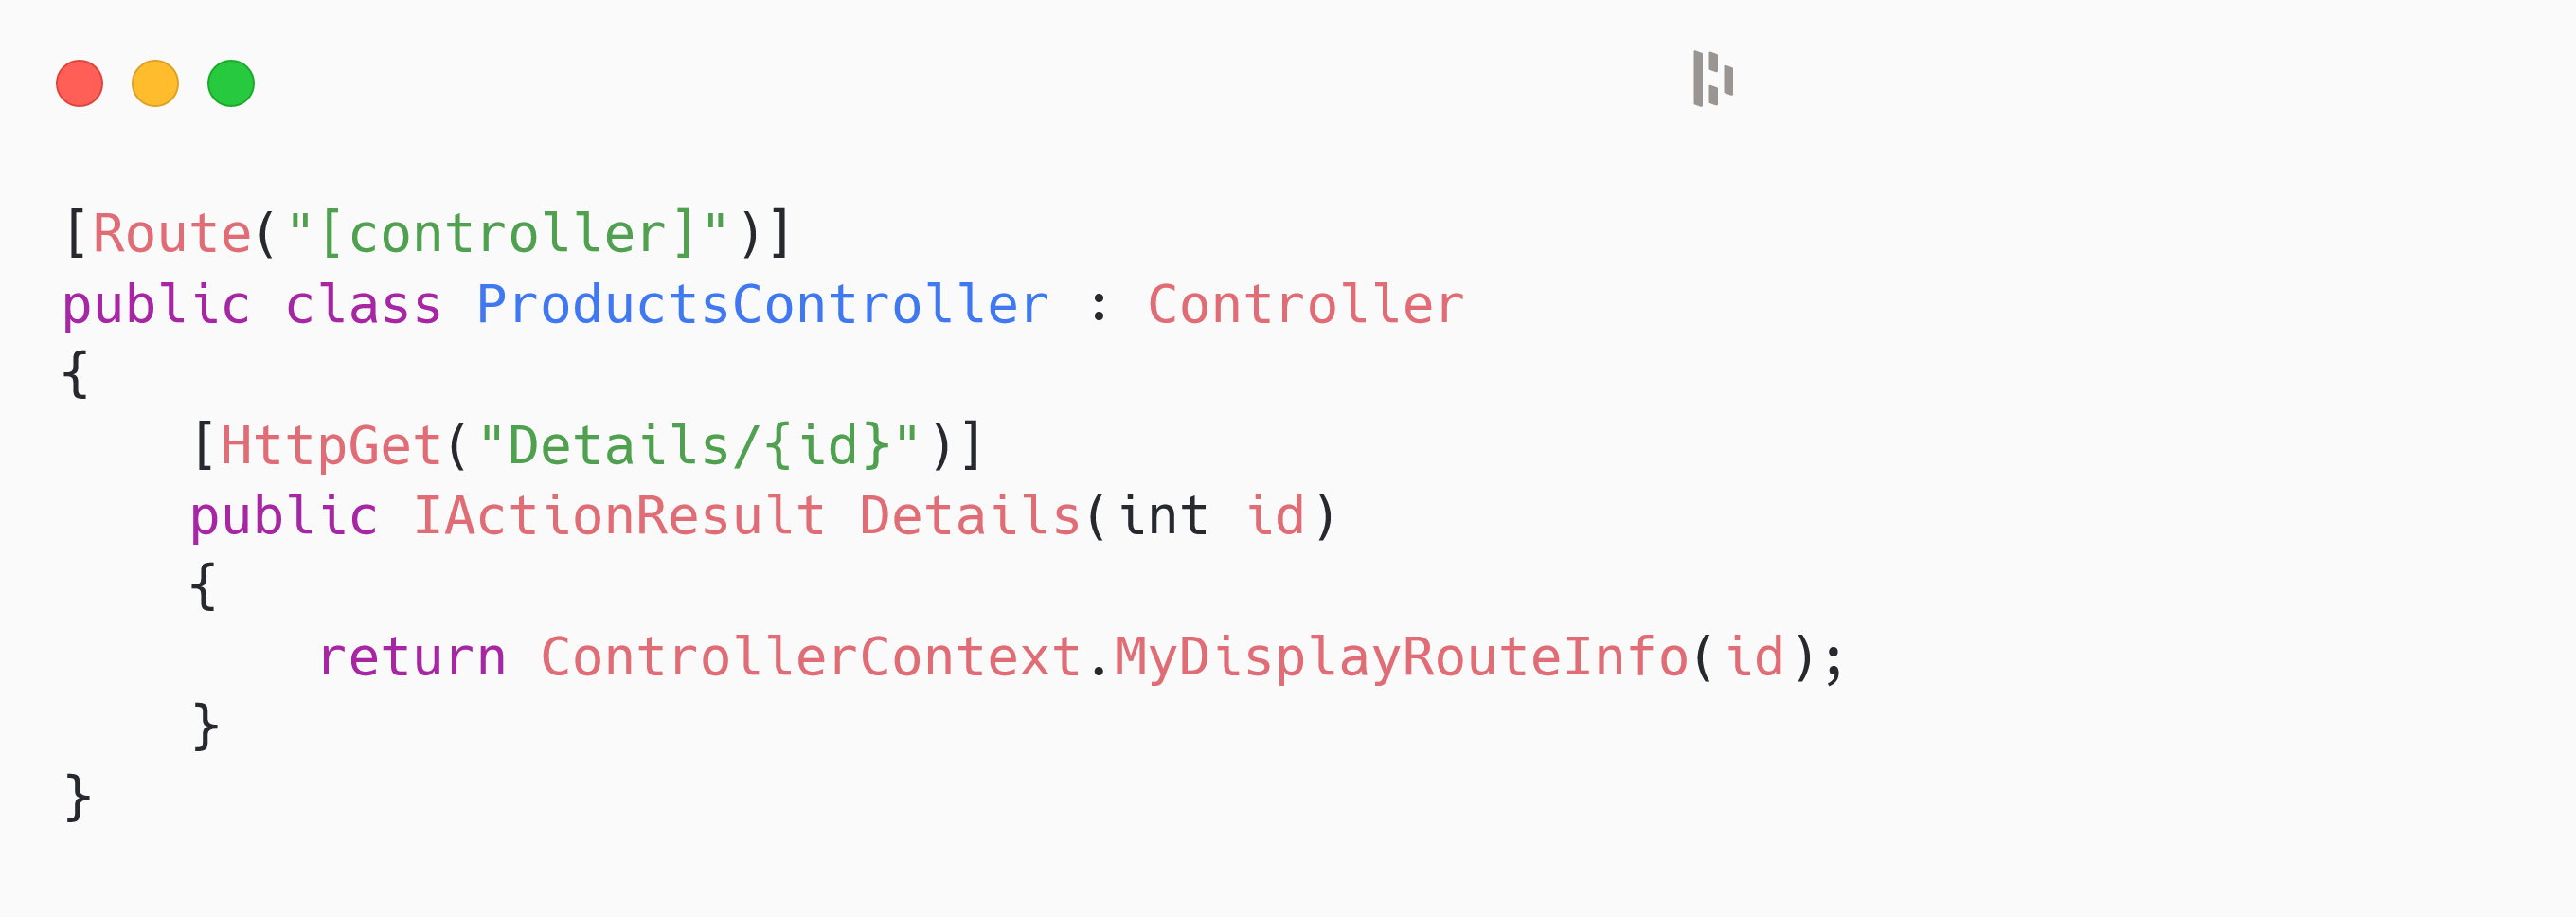
\includegraphics[width=1\textwidth]{graphics/attribute-routing.png}
\caption{An example controller using attributes in ASP.NET Core}
\label{fig:controller}
\end{figure}

In ASP.NET Core, endpoint mapping automation, also known as "action discovery," is achieved by dynamically scanning the entire codebase during the startup phase of the application. However, this dynamic action discovery relies on certain services and middleware incorporated into the application at different stages of the startup phase. Figure \ref{fig:startup-phase} shows the startup phase of an ASP.NET Core application and the order of adding services and middleware.

\begin{figure}[H]
\centering
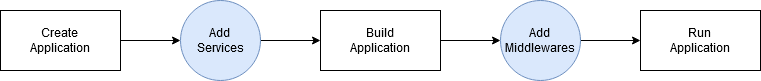
\includegraphics[width=1\textwidth]{graphics/startup-phase.png}
\caption{Flow of the application startup process in ASP.NET Core}
\label{fig:startup-phase}
\end{figure}

ASP.NET Core follows a specific sequence during application setup:

\begin{enumerate}
    \item An application is created, and required services are added to the Dependency Injection (DI) container. Classes can then define their dependencies in their constructor, and the DI container automatically resolves these dependencies to the right implementation.
    \item The application is built, incorporating the registered services.
    \item Middlewares are added. These components have the power to influence how an ASP.NET Core application handles each request.
    \item The application is started.
\end{enumerate}

In this startup sequence, the dynamic action discovery happens before the application is started and involves a middleware and a mapper. The middleware in question is the routing middleware, which relies on the mapper's output to route requests to the correct actions.

The mapper is invoked when using methods like \verb|MapControllers|, which generate the application model—a representation of all controllers and their actions in the application. The process is visualized in Figure \ref{fig:sequence-diagram} as a sequence diagram.

\begin{figure}[H]
\centering
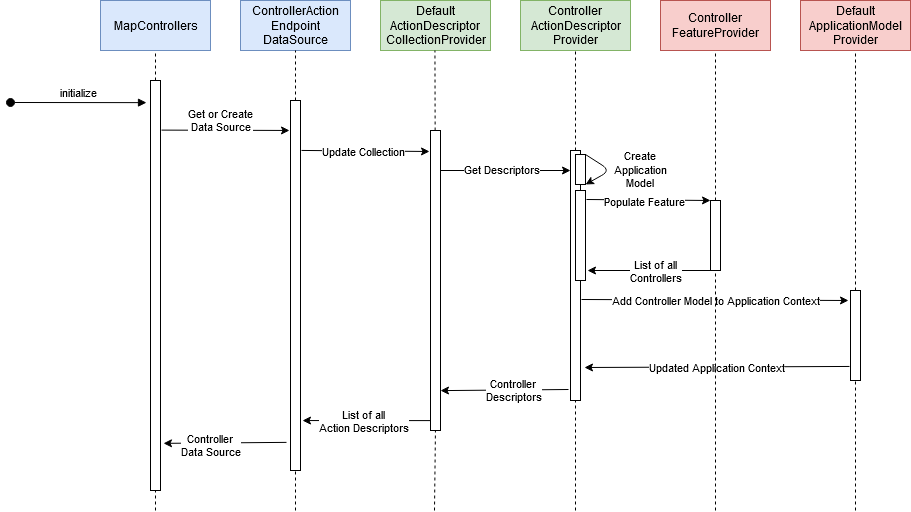
\includegraphics[width=1\textwidth]{graphics/Sequence Diagram.drawio.png}
\caption{Sequence diagram illustrating the application model creation process}
\label{fig:sequence-diagram}
\end{figure}

The sequence of operations leading to action discovery in ASP.NET Core begins when a developer calls the mapping method, such as \verb|MapControllers|. This method, identified in blue in Figure \ref{fig:sequence-diagram}, initiates the process of endpoint mapping.

Upon invocation, \verb|MapControllers| creates an instance of the \verb|ControllerActionEndpointDataSource| (highlighted in blue). This class is responsible for generating a collection of endpoints, which form the building blocks of the application's routing mechanism. Each endpoint encapsulates essential information, such as the target action (method) to be executed upon a specific user request.

In order to generate this collection of endpoints, the \verb|ControllerActionEndpointDataSource| class needs to obtain an overview of all available actions in the application. For this, it requests an \verb|IActionDescriptorCollectionProvider| from the DI container. Per default, this resolves to the \verb|DefaultActionDescriptorCollectionProvider|. It then indirectly calls the \verb|UpdateCollection| method of the \verb|DefaultActionDescriptorCollectionProvider|. This action description provider fetches all the registered \verb|ActionDescriptorProvider| services from the DI container and executes them, thereby gathering actions from a range of sources.

One specific '\verb|ActionDescriptorProvider| service of interest here is the \verb|ControllerActionDescriptorProvider| (marked in green). This service holds the key to our focus area: the actions located within the application's controllers. This service initiates the process of creating an application model—a comprehensive representation of all controller-related information.

The \verb|ControllerActionDescriptorProvider| works through three sequential phases:

\begin{enumerate}
    \item \textbf{Creation of an Application Model}: An empty application model is initialized. This model is designed to hold all relevant information about the controllers in the application and their associated actions.

    \item \textbf{Controller Discovery}: The \verb|ControllerActionDescriptorProvider| calls all available \verb|FeatureProviders| in the DI container, which by default is only the \verb|ControllerFeatureProvider| (marked red). The \verb|ControllerActionDescriptorProvider| then calls the \verb|PopulateFeature| method of every \verb|FeatureProvider| to identify all controllers within the application. The \verb|ControllerFeatureProvider| scans all application parts, which are assemblies that reference the MVC package from ASP.NET Core and could therefore contain controllers. This means that by default, all dependencies that use the MVC package, like Swagger, are analyzed as well. Using reflection, the \verb|PopulateFeature| method analyzes all classes within these assemblies using reflection, extracting those that qualify as controller classes. These discovered controllers are then added to the application model.

    \item \textbf{Model Population}: The \verb|ControllerActionDescriptorProvider| proceeds to call all available \verb|ApplicationModelProviders| in the DI container. These providers populate the application model with detailed information about the actions within each identified controller. The most important \verb|ApplicationModelProvider| is the \verb|DefaultApplicationModelProvider| (marked red) which loops over the found controllers and extracts their actions along with any associated attributes. The service then creates 'selectors' for each action that holds information about the action's route, the HTTP method (GET, POST, DELETE, etc.), a unique name for the action, and other relevant metadata.
\end{enumerate}

After these three phases, the \verb|ControllerActionDescriptorProvider| has effectively created an application model containing all the information about the controllers of the application. This model is sent back up the call stack to the \verb|MapControllers| method, which compiles this information into Endpoint objects. The routing mechanism uses these endpoint objects to appropriately route incoming requests to the correct actions.

The key takeaway is that the services marked in red in Figure \ref{fig:sequence-diagram}—the \verb|ControllerFeatureProvider|, and \verb|DefaultApplicationModelProvider|—play crucial roles in dynamic action discovery and need to be replaced for static action discovery. The objects marked in blue represent objects that are either directly called by the developer or instantiated without dependency injection and can not be modified. The green objects represent services that can be modified by changing the implementation in the DI container but do not use reflection and therefore do not need to be modified by the static action discovery. Optimizing the startup performance of the application involves substituting the services marked red with custom implementations of the same interfaces designed to employ static action discovery. The creation of the static action discovery is the focus of the next chapter.